\documentclass[11pt]{article}

    \usepackage[breakable]{tcolorbox}
    \usepackage{parskip} % Stop auto-indenting (to mimic markdown behaviour)
    
    \usepackage{iftex}
    \ifPDFTeX
    	\usepackage[T1]{fontenc}
    	\usepackage{mathpazo}
    \else
    	\usepackage{fontspec}
    \fi

    % Basic figure setup, for now with no caption control since it's done
    % automatically by Pandoc (which extracts ![](path) syntax from Markdown).
    \usepackage{graphicx}
    % Maintain compatibility with old templates. Remove in nbconvert 6.0
    \let\Oldincludegraphics\includegraphics
    % Ensure that by default, figures have no caption (until we provide a
    % proper Figure object with a Caption API and a way to capture that
    % in the conversion process - todo).
    \usepackage{caption}
    \DeclareCaptionFormat{nocaption}{}
    \captionsetup{format=nocaption,aboveskip=0pt,belowskip=0pt}

    \usepackage[Export]{adjustbox} % Used to constrain images to a maximum size
    \adjustboxset{max size={0.9\linewidth}{0.9\paperheight}}
    \usepackage{float}
    \floatplacement{figure}{H} % forces figures to be placed at the correct location
    \usepackage{xcolor} % Allow colors to be defined
    \usepackage{enumerate} % Needed for markdown enumerations to work
    \usepackage{geometry} % Used to adjust the document margins
    \usepackage{amsmath} % Equations
    \usepackage{amssymb} % Equations
    \usepackage{textcomp} % defines textquotesingle
    % Hack from http://tex.stackexchange.com/a/47451/13684:
    \AtBeginDocument{%
        \def\PYZsq{\textquotesingle}% Upright quotes in Pygmentized code
    }
    \usepackage{upquote} % Upright quotes for verbatim code
    \usepackage{eurosym} % defines \euro
    \usepackage[mathletters]{ucs} % Extended unicode (utf-8) support
    \usepackage{fancyvrb} % verbatim replacement that allows latex
    \usepackage{grffile} % extends the file name processing of package graphics 
                         % to support a larger range
    \makeatletter % fix for grffile with XeLaTeX
    \def\Gread@@xetex#1{%
      \IfFileExists{"\Gin@base".bb}%
      {\Gread@eps{\Gin@base.bb}}%
      {\Gread@@xetex@aux#1}%
    }
    \makeatother

    % The hyperref package gives us a pdf with properly built
    % internal navigation ('pdf bookmarks' for the table of contents,
    % internal cross-reference links, web links for URLs, etc.)
    \usepackage{hyperref}
    % The default LaTeX title has an obnoxious amount of whitespace. By default,
    % titling removes some of it. It also provides customization options.
    \usepackage{titling}
    \usepackage{longtable} % longtable support required by pandoc >1.10
    \usepackage{booktabs}  % table support for pandoc > 1.12.2
    \usepackage[inline]{enumitem} % IRkernel/repr support (it uses the enumerate* environment)
    \usepackage[normalem]{ulem} % ulem is needed to support strikethroughs (\sout)
                                % normalem makes italics be italics, not underlines
    \usepackage{mathrsfs}
    

    
    % Colors for the hyperref package
    \definecolor{urlcolor}{rgb}{0,.145,.698}
    \definecolor{linkcolor}{rgb}{.71,0.21,0.01}
    \definecolor{citecolor}{rgb}{.12,.54,.11}

    % ANSI colors
    \definecolor{ansi-black}{HTML}{3E424D}
    \definecolor{ansi-black-intense}{HTML}{282C36}
    \definecolor{ansi-red}{HTML}{E75C58}
    \definecolor{ansi-red-intense}{HTML}{B22B31}
    \definecolor{ansi-green}{HTML}{00A250}
    \definecolor{ansi-green-intense}{HTML}{007427}
    \definecolor{ansi-yellow}{HTML}{DDB62B}
    \definecolor{ansi-yellow-intense}{HTML}{B27D12}
    \definecolor{ansi-blue}{HTML}{208FFB}
    \definecolor{ansi-blue-intense}{HTML}{0065CA}
    \definecolor{ansi-magenta}{HTML}{D160C4}
    \definecolor{ansi-magenta-intense}{HTML}{A03196}
    \definecolor{ansi-cyan}{HTML}{60C6C8}
    \definecolor{ansi-cyan-intense}{HTML}{258F8F}
    \definecolor{ansi-white}{HTML}{C5C1B4}
    \definecolor{ansi-white-intense}{HTML}{A1A6B2}
    \definecolor{ansi-default-inverse-fg}{HTML}{FFFFFF}
    \definecolor{ansi-default-inverse-bg}{HTML}{000000}

    % commands and environments needed by pandoc snippets
    % extracted from the output of `pandoc -s`
    \providecommand{\tightlist}{%
      \setlength{\itemsep}{0pt}\setlength{\parskip}{0pt}}
    \DefineVerbatimEnvironment{Highlighting}{Verbatim}{commandchars=\\\{\}}
    % Add ',fontsize=\small' for more characters per line
    \newenvironment{Shaded}{}{}
    \newcommand{\KeywordTok}[1]{\textcolor[rgb]{0.00,0.44,0.13}{\textbf{{#1}}}}
    \newcommand{\DataTypeTok}[1]{\textcolor[rgb]{0.56,0.13,0.00}{{#1}}}
    \newcommand{\DecValTok}[1]{\textcolor[rgb]{0.25,0.63,0.44}{{#1}}}
    \newcommand{\BaseNTok}[1]{\textcolor[rgb]{0.25,0.63,0.44}{{#1}}}
    \newcommand{\FloatTok}[1]{\textcolor[rgb]{0.25,0.63,0.44}{{#1}}}
    \newcommand{\CharTok}[1]{\textcolor[rgb]{0.25,0.44,0.63}{{#1}}}
    \newcommand{\StringTok}[1]{\textcolor[rgb]{0.25,0.44,0.63}{{#1}}}
    \newcommand{\CommentTok}[1]{\textcolor[rgb]{0.38,0.63,0.69}{\textit{{#1}}}}
    \newcommand{\OtherTok}[1]{\textcolor[rgb]{0.00,0.44,0.13}{{#1}}}
    \newcommand{\AlertTok}[1]{\textcolor[rgb]{1.00,0.00,0.00}{\textbf{{#1}}}}
    \newcommand{\FunctionTok}[1]{\textcolor[rgb]{0.02,0.16,0.49}{{#1}}}
    \newcommand{\RegionMarkerTok}[1]{{#1}}
    \newcommand{\ErrorTok}[1]{\textcolor[rgb]{1.00,0.00,0.00}{\textbf{{#1}}}}
    \newcommand{\NormalTok}[1]{{#1}}
    
    % Additional commands for more recent versions of Pandoc
    \newcommand{\ConstantTok}[1]{\textcolor[rgb]{0.53,0.00,0.00}{{#1}}}
    \newcommand{\SpecialCharTok}[1]{\textcolor[rgb]{0.25,0.44,0.63}{{#1}}}
    \newcommand{\VerbatimStringTok}[1]{\textcolor[rgb]{0.25,0.44,0.63}{{#1}}}
    \newcommand{\SpecialStringTok}[1]{\textcolor[rgb]{0.73,0.40,0.53}{{#1}}}
    \newcommand{\ImportTok}[1]{{#1}}
    \newcommand{\DocumentationTok}[1]{\textcolor[rgb]{0.73,0.13,0.13}{\textit{{#1}}}}
    \newcommand{\AnnotationTok}[1]{\textcolor[rgb]{0.38,0.63,0.69}{\textbf{\textit{{#1}}}}}
    \newcommand{\CommentVarTok}[1]{\textcolor[rgb]{0.38,0.63,0.69}{\textbf{\textit{{#1}}}}}
    \newcommand{\VariableTok}[1]{\textcolor[rgb]{0.10,0.09,0.49}{{#1}}}
    \newcommand{\ControlFlowTok}[1]{\textcolor[rgb]{0.00,0.44,0.13}{\textbf{{#1}}}}
    \newcommand{\OperatorTok}[1]{\textcolor[rgb]{0.40,0.40,0.40}{{#1}}}
    \newcommand{\BuiltInTok}[1]{{#1}}
    \newcommand{\ExtensionTok}[1]{{#1}}
    \newcommand{\PreprocessorTok}[1]{\textcolor[rgb]{0.74,0.48,0.00}{{#1}}}
    \newcommand{\AttributeTok}[1]{\textcolor[rgb]{0.49,0.56,0.16}{{#1}}}
    \newcommand{\InformationTok}[1]{\textcolor[rgb]{0.38,0.63,0.69}{\textbf{\textit{{#1}}}}}
    \newcommand{\WarningTok}[1]{\textcolor[rgb]{0.38,0.63,0.69}{\textbf{\textit{{#1}}}}}
    
    
    % Define a nice break command that doesn't care if a line doesn't already
    % exist.
    \def\br{\hspace*{\fill} \\* }
    % Math Jax compatibility definitions
    \def\gt{>}
    \def\lt{<}
    \let\Oldtex\TeX
    \let\Oldlatex\LaTeX
    \renewcommand{\TeX}{\textrm{\Oldtex}}
    \renewcommand{\LaTeX}{\textrm{\Oldlatex}}
    % Document parameters
    % Document title
    \title{improving-machine-learning-experience}
    
    
    
    
    
% Pygments definitions
\makeatletter
\def\PY@reset{\let\PY@it=\relax \let\PY@bf=\relax%
    \let\PY@ul=\relax \let\PY@tc=\relax%
    \let\PY@bc=\relax \let\PY@ff=\relax}
\def\PY@tok#1{\csname PY@tok@#1\endcsname}
\def\PY@toks#1+{\ifx\relax#1\empty\else%
    \PY@tok{#1}\expandafter\PY@toks\fi}
\def\PY@do#1{\PY@bc{\PY@tc{\PY@ul{%
    \PY@it{\PY@bf{\PY@ff{#1}}}}}}}
\def\PY#1#2{\PY@reset\PY@toks#1+\relax+\PY@do{#2}}

\expandafter\def\csname PY@tok@w\endcsname{\def\PY@tc##1{\textcolor[rgb]{0.73,0.73,0.73}{##1}}}
\expandafter\def\csname PY@tok@c\endcsname{\let\PY@it=\textit\def\PY@tc##1{\textcolor[rgb]{0.25,0.50,0.50}{##1}}}
\expandafter\def\csname PY@tok@cp\endcsname{\def\PY@tc##1{\textcolor[rgb]{0.74,0.48,0.00}{##1}}}
\expandafter\def\csname PY@tok@k\endcsname{\let\PY@bf=\textbf\def\PY@tc##1{\textcolor[rgb]{0.00,0.50,0.00}{##1}}}
\expandafter\def\csname PY@tok@kp\endcsname{\def\PY@tc##1{\textcolor[rgb]{0.00,0.50,0.00}{##1}}}
\expandafter\def\csname PY@tok@kt\endcsname{\def\PY@tc##1{\textcolor[rgb]{0.69,0.00,0.25}{##1}}}
\expandafter\def\csname PY@tok@o\endcsname{\def\PY@tc##1{\textcolor[rgb]{0.40,0.40,0.40}{##1}}}
\expandafter\def\csname PY@tok@ow\endcsname{\let\PY@bf=\textbf\def\PY@tc##1{\textcolor[rgb]{0.67,0.13,1.00}{##1}}}
\expandafter\def\csname PY@tok@nb\endcsname{\def\PY@tc##1{\textcolor[rgb]{0.00,0.50,0.00}{##1}}}
\expandafter\def\csname PY@tok@nf\endcsname{\def\PY@tc##1{\textcolor[rgb]{0.00,0.00,1.00}{##1}}}
\expandafter\def\csname PY@tok@nc\endcsname{\let\PY@bf=\textbf\def\PY@tc##1{\textcolor[rgb]{0.00,0.00,1.00}{##1}}}
\expandafter\def\csname PY@tok@nn\endcsname{\let\PY@bf=\textbf\def\PY@tc##1{\textcolor[rgb]{0.00,0.00,1.00}{##1}}}
\expandafter\def\csname PY@tok@ne\endcsname{\let\PY@bf=\textbf\def\PY@tc##1{\textcolor[rgb]{0.82,0.25,0.23}{##1}}}
\expandafter\def\csname PY@tok@nv\endcsname{\def\PY@tc##1{\textcolor[rgb]{0.10,0.09,0.49}{##1}}}
\expandafter\def\csname PY@tok@no\endcsname{\def\PY@tc##1{\textcolor[rgb]{0.53,0.00,0.00}{##1}}}
\expandafter\def\csname PY@tok@nl\endcsname{\def\PY@tc##1{\textcolor[rgb]{0.63,0.63,0.00}{##1}}}
\expandafter\def\csname PY@tok@ni\endcsname{\let\PY@bf=\textbf\def\PY@tc##1{\textcolor[rgb]{0.60,0.60,0.60}{##1}}}
\expandafter\def\csname PY@tok@na\endcsname{\def\PY@tc##1{\textcolor[rgb]{0.49,0.56,0.16}{##1}}}
\expandafter\def\csname PY@tok@nt\endcsname{\let\PY@bf=\textbf\def\PY@tc##1{\textcolor[rgb]{0.00,0.50,0.00}{##1}}}
\expandafter\def\csname PY@tok@nd\endcsname{\def\PY@tc##1{\textcolor[rgb]{0.67,0.13,1.00}{##1}}}
\expandafter\def\csname PY@tok@s\endcsname{\def\PY@tc##1{\textcolor[rgb]{0.73,0.13,0.13}{##1}}}
\expandafter\def\csname PY@tok@sd\endcsname{\let\PY@it=\textit\def\PY@tc##1{\textcolor[rgb]{0.73,0.13,0.13}{##1}}}
\expandafter\def\csname PY@tok@si\endcsname{\let\PY@bf=\textbf\def\PY@tc##1{\textcolor[rgb]{0.73,0.40,0.53}{##1}}}
\expandafter\def\csname PY@tok@se\endcsname{\let\PY@bf=\textbf\def\PY@tc##1{\textcolor[rgb]{0.73,0.40,0.13}{##1}}}
\expandafter\def\csname PY@tok@sr\endcsname{\def\PY@tc##1{\textcolor[rgb]{0.73,0.40,0.53}{##1}}}
\expandafter\def\csname PY@tok@ss\endcsname{\def\PY@tc##1{\textcolor[rgb]{0.10,0.09,0.49}{##1}}}
\expandafter\def\csname PY@tok@sx\endcsname{\def\PY@tc##1{\textcolor[rgb]{0.00,0.50,0.00}{##1}}}
\expandafter\def\csname PY@tok@m\endcsname{\def\PY@tc##1{\textcolor[rgb]{0.40,0.40,0.40}{##1}}}
\expandafter\def\csname PY@tok@gh\endcsname{\let\PY@bf=\textbf\def\PY@tc##1{\textcolor[rgb]{0.00,0.00,0.50}{##1}}}
\expandafter\def\csname PY@tok@gu\endcsname{\let\PY@bf=\textbf\def\PY@tc##1{\textcolor[rgb]{0.50,0.00,0.50}{##1}}}
\expandafter\def\csname PY@tok@gd\endcsname{\def\PY@tc##1{\textcolor[rgb]{0.63,0.00,0.00}{##1}}}
\expandafter\def\csname PY@tok@gi\endcsname{\def\PY@tc##1{\textcolor[rgb]{0.00,0.63,0.00}{##1}}}
\expandafter\def\csname PY@tok@gr\endcsname{\def\PY@tc##1{\textcolor[rgb]{1.00,0.00,0.00}{##1}}}
\expandafter\def\csname PY@tok@ge\endcsname{\let\PY@it=\textit}
\expandafter\def\csname PY@tok@gs\endcsname{\let\PY@bf=\textbf}
\expandafter\def\csname PY@tok@gp\endcsname{\let\PY@bf=\textbf\def\PY@tc##1{\textcolor[rgb]{0.00,0.00,0.50}{##1}}}
\expandafter\def\csname PY@tok@go\endcsname{\def\PY@tc##1{\textcolor[rgb]{0.53,0.53,0.53}{##1}}}
\expandafter\def\csname PY@tok@gt\endcsname{\def\PY@tc##1{\textcolor[rgb]{0.00,0.27,0.87}{##1}}}
\expandafter\def\csname PY@tok@err\endcsname{\def\PY@bc##1{\setlength{\fboxsep}{0pt}\fcolorbox[rgb]{1.00,0.00,0.00}{1,1,1}{\strut ##1}}}
\expandafter\def\csname PY@tok@kc\endcsname{\let\PY@bf=\textbf\def\PY@tc##1{\textcolor[rgb]{0.00,0.50,0.00}{##1}}}
\expandafter\def\csname PY@tok@kd\endcsname{\let\PY@bf=\textbf\def\PY@tc##1{\textcolor[rgb]{0.00,0.50,0.00}{##1}}}
\expandafter\def\csname PY@tok@kn\endcsname{\let\PY@bf=\textbf\def\PY@tc##1{\textcolor[rgb]{0.00,0.50,0.00}{##1}}}
\expandafter\def\csname PY@tok@kr\endcsname{\let\PY@bf=\textbf\def\PY@tc##1{\textcolor[rgb]{0.00,0.50,0.00}{##1}}}
\expandafter\def\csname PY@tok@bp\endcsname{\def\PY@tc##1{\textcolor[rgb]{0.00,0.50,0.00}{##1}}}
\expandafter\def\csname PY@tok@fm\endcsname{\def\PY@tc##1{\textcolor[rgb]{0.00,0.00,1.00}{##1}}}
\expandafter\def\csname PY@tok@vc\endcsname{\def\PY@tc##1{\textcolor[rgb]{0.10,0.09,0.49}{##1}}}
\expandafter\def\csname PY@tok@vg\endcsname{\def\PY@tc##1{\textcolor[rgb]{0.10,0.09,0.49}{##1}}}
\expandafter\def\csname PY@tok@vi\endcsname{\def\PY@tc##1{\textcolor[rgb]{0.10,0.09,0.49}{##1}}}
\expandafter\def\csname PY@tok@vm\endcsname{\def\PY@tc##1{\textcolor[rgb]{0.10,0.09,0.49}{##1}}}
\expandafter\def\csname PY@tok@sa\endcsname{\def\PY@tc##1{\textcolor[rgb]{0.73,0.13,0.13}{##1}}}
\expandafter\def\csname PY@tok@sb\endcsname{\def\PY@tc##1{\textcolor[rgb]{0.73,0.13,0.13}{##1}}}
\expandafter\def\csname PY@tok@sc\endcsname{\def\PY@tc##1{\textcolor[rgb]{0.73,0.13,0.13}{##1}}}
\expandafter\def\csname PY@tok@dl\endcsname{\def\PY@tc##1{\textcolor[rgb]{0.73,0.13,0.13}{##1}}}
\expandafter\def\csname PY@tok@s2\endcsname{\def\PY@tc##1{\textcolor[rgb]{0.73,0.13,0.13}{##1}}}
\expandafter\def\csname PY@tok@sh\endcsname{\def\PY@tc##1{\textcolor[rgb]{0.73,0.13,0.13}{##1}}}
\expandafter\def\csname PY@tok@s1\endcsname{\def\PY@tc##1{\textcolor[rgb]{0.73,0.13,0.13}{##1}}}
\expandafter\def\csname PY@tok@mb\endcsname{\def\PY@tc##1{\textcolor[rgb]{0.40,0.40,0.40}{##1}}}
\expandafter\def\csname PY@tok@mf\endcsname{\def\PY@tc##1{\textcolor[rgb]{0.40,0.40,0.40}{##1}}}
\expandafter\def\csname PY@tok@mh\endcsname{\def\PY@tc##1{\textcolor[rgb]{0.40,0.40,0.40}{##1}}}
\expandafter\def\csname PY@tok@mi\endcsname{\def\PY@tc##1{\textcolor[rgb]{0.40,0.40,0.40}{##1}}}
\expandafter\def\csname PY@tok@il\endcsname{\def\PY@tc##1{\textcolor[rgb]{0.40,0.40,0.40}{##1}}}
\expandafter\def\csname PY@tok@mo\endcsname{\def\PY@tc##1{\textcolor[rgb]{0.40,0.40,0.40}{##1}}}
\expandafter\def\csname PY@tok@ch\endcsname{\let\PY@it=\textit\def\PY@tc##1{\textcolor[rgb]{0.25,0.50,0.50}{##1}}}
\expandafter\def\csname PY@tok@cm\endcsname{\let\PY@it=\textit\def\PY@tc##1{\textcolor[rgb]{0.25,0.50,0.50}{##1}}}
\expandafter\def\csname PY@tok@cpf\endcsname{\let\PY@it=\textit\def\PY@tc##1{\textcolor[rgb]{0.25,0.50,0.50}{##1}}}
\expandafter\def\csname PY@tok@c1\endcsname{\let\PY@it=\textit\def\PY@tc##1{\textcolor[rgb]{0.25,0.50,0.50}{##1}}}
\expandafter\def\csname PY@tok@cs\endcsname{\let\PY@it=\textit\def\PY@tc##1{\textcolor[rgb]{0.25,0.50,0.50}{##1}}}

\def\PYZbs{\char`\\}
\def\PYZus{\char`\_}
\def\PYZob{\char`\{}
\def\PYZcb{\char`\}}
\def\PYZca{\char`\^}
\def\PYZam{\char`\&}
\def\PYZlt{\char`\<}
\def\PYZgt{\char`\>}
\def\PYZsh{\char`\#}
\def\PYZpc{\char`\%}
\def\PYZdl{\char`\$}
\def\PYZhy{\char`\-}
\def\PYZsq{\char`\'}
\def\PYZdq{\char`\"}
\def\PYZti{\char`\~}
% for compatibility with earlier versions
\def\PYZat{@}
\def\PYZlb{[}
\def\PYZrb{]}
\makeatother


    % For linebreaks inside Verbatim environment from package fancyvrb. 
    \makeatletter
        \newbox\Wrappedcontinuationbox 
        \newbox\Wrappedvisiblespacebox 
        \newcommand*\Wrappedvisiblespace {\textcolor{red}{\textvisiblespace}} 
        \newcommand*\Wrappedcontinuationsymbol {\textcolor{red}{\llap{\tiny$\m@th\hookrightarrow$}}} 
        \newcommand*\Wrappedcontinuationindent {3ex } 
        \newcommand*\Wrappedafterbreak {\kern\Wrappedcontinuationindent\copy\Wrappedcontinuationbox} 
        % Take advantage of the already applied Pygments mark-up to insert 
        % potential linebreaks for TeX processing. 
        %        {, <, #, %, $, ' and ": go to next line. 
        %        _, }, ^, &, >, - and ~: stay at end of broken line. 
        % Use of \textquotesingle for straight quote. 
        \newcommand*\Wrappedbreaksatspecials {% 
            \def\PYGZus{\discretionary{\char`\_}{\Wrappedafterbreak}{\char`\_}}% 
            \def\PYGZob{\discretionary{}{\Wrappedafterbreak\char`\{}{\char`\{}}% 
            \def\PYGZcb{\discretionary{\char`\}}{\Wrappedafterbreak}{\char`\}}}% 
            \def\PYGZca{\discretionary{\char`\^}{\Wrappedafterbreak}{\char`\^}}% 
            \def\PYGZam{\discretionary{\char`\&}{\Wrappedafterbreak}{\char`\&}}% 
            \def\PYGZlt{\discretionary{}{\Wrappedafterbreak\char`\<}{\char`\<}}% 
            \def\PYGZgt{\discretionary{\char`\>}{\Wrappedafterbreak}{\char`\>}}% 
            \def\PYGZsh{\discretionary{}{\Wrappedafterbreak\char`\#}{\char`\#}}% 
            \def\PYGZpc{\discretionary{}{\Wrappedafterbreak\char`\%}{\char`\%}}% 
            \def\PYGZdl{\discretionary{}{\Wrappedafterbreak\char`\$}{\char`\$}}% 
            \def\PYGZhy{\discretionary{\char`\-}{\Wrappedafterbreak}{\char`\-}}% 
            \def\PYGZsq{\discretionary{}{\Wrappedafterbreak\textquotesingle}{\textquotesingle}}% 
            \def\PYGZdq{\discretionary{}{\Wrappedafterbreak\char`\"}{\char`\"}}% 
            \def\PYGZti{\discretionary{\char`\~}{\Wrappedafterbreak}{\char`\~}}% 
        } 
        % Some characters . , ; ? ! / are not pygmentized. 
        % This macro makes them "active" and they will insert potential linebreaks 
        \newcommand*\Wrappedbreaksatpunct {% 
            \lccode`\~`\.\lowercase{\def~}{\discretionary{\hbox{\char`\.}}{\Wrappedafterbreak}{\hbox{\char`\.}}}% 
            \lccode`\~`\,\lowercase{\def~}{\discretionary{\hbox{\char`\,}}{\Wrappedafterbreak}{\hbox{\char`\,}}}% 
            \lccode`\~`\;\lowercase{\def~}{\discretionary{\hbox{\char`\;}}{\Wrappedafterbreak}{\hbox{\char`\;}}}% 
            \lccode`\~`\:\lowercase{\def~}{\discretionary{\hbox{\char`\:}}{\Wrappedafterbreak}{\hbox{\char`\:}}}% 
            \lccode`\~`\?\lowercase{\def~}{\discretionary{\hbox{\char`\?}}{\Wrappedafterbreak}{\hbox{\char`\?}}}% 
            \lccode`\~`\!\lowercase{\def~}{\discretionary{\hbox{\char`\!}}{\Wrappedafterbreak}{\hbox{\char`\!}}}% 
            \lccode`\~`\/\lowercase{\def~}{\discretionary{\hbox{\char`\/}}{\Wrappedafterbreak}{\hbox{\char`\/}}}% 
            \catcode`\.\active
            \catcode`\,\active 
            \catcode`\;\active
            \catcode`\:\active
            \catcode`\?\active
            \catcode`\!\active
            \catcode`\/\active 
            \lccode`\~`\~ 	
        }
    \makeatother

    \let\OriginalVerbatim=\Verbatim
    \makeatletter
    \renewcommand{\Verbatim}[1][1]{%
        %\parskip\z@skip
        \sbox\Wrappedcontinuationbox {\Wrappedcontinuationsymbol}%
        \sbox\Wrappedvisiblespacebox {\FV@SetupFont\Wrappedvisiblespace}%
        \def\FancyVerbFormatLine ##1{\hsize\linewidth
            \vtop{\raggedright\hyphenpenalty\z@\exhyphenpenalty\z@
                \doublehyphendemerits\z@\finalhyphendemerits\z@
                \strut ##1\strut}%
        }%
        % If the linebreak is at a space, the latter will be displayed as visible
        % space at end of first line, and a continuation symbol starts next line.
        % Stretch/shrink are however usually zero for typewriter font.
        \def\FV@Space {%
            \nobreak\hskip\z@ plus\fontdimen3\font minus\fontdimen4\font
            \discretionary{\copy\Wrappedvisiblespacebox}{\Wrappedafterbreak}
            {\kern\fontdimen2\font}%
        }%
        
        % Allow breaks at special characters using \PYG... macros.
        \Wrappedbreaksatspecials
        % Breaks at punctuation characters . , ; ? ! and / need catcode=\active 	
        \OriginalVerbatim[#1,codes*=\Wrappedbreaksatpunct]%
    }
    \makeatother

    % Exact colors from NB
    \definecolor{incolor}{HTML}{303F9F}
    \definecolor{outcolor}{HTML}{D84315}
    \definecolor{cellborder}{HTML}{CFCFCF}
    \definecolor{cellbackground}{HTML}{F7F7F7}
    
    % prompt
    \makeatletter
    \newcommand{\boxspacing}{\kern\kvtcb@left@rule\kern\kvtcb@boxsep}
    \makeatother
    \newcommand{\prompt}[4]{
        \ttfamily\llap{{\color{#2}[#3]:\hspace{3pt}#4}}\vspace{-\baselineskip}
    }
    

    
    % Prevent overflowing lines due to hard-to-break entities
    \sloppy 
    % Setup hyperref package
    \hypersetup{
      breaklinks=true,  % so long urls are correctly broken across lines
      colorlinks=true,
      urlcolor=urlcolor,
      linkcolor=linkcolor,
      citecolor=citecolor,
      }
    % Slightly bigger margins than the latex defaults
    
    \geometry{verbose,tmargin=1in,bmargin=1in,lmargin=1in,rmargin=1in}
    
    

\begin{document}
    
    \maketitle
    
    

    
    \section{Improving Machine Learning Experience With Multimedia
Techniques}\label{improving-machine-learning-experience-with-multimedia-techniques}

Marco A. Franchi

\subsection{\texorpdfstring{\emph{Abstract}}{Abstract}}\label{abstract}

\emph{It has been very common face machine learning algorithms at the
multimedia area: traffic count; real-time vigilance cameras; baggage
tracker; face/expression recognition; and so on. It is so common that it
was designed a name for it, Machine Vision. However, it is perceptive
the gap between machine learning and multimedia solutions, where even at
simple embedded systems it is possible to reach 4k videos running at 60
frames per second, whereas the best neural network solution only handles
224x224 frames at 300 milliseconds in the same system. Due to this gap,
a vast number of solutions as being developed: dedicated hardware for
inference process; model manipulation; accelerated pre-processing image
solutions; and video manipulation techniques. This paper is based at the
study of these videos manipulation techniques, exposing the most common
algorithmics, such as frame-skip, frame-droop, resizing, color convert,
and overlay solutions; and showing the main difference between them,
when the solution can be applied, and the expected performance for each
one.}

\subsection{Introduction}\label{introduction}

Aiming to diminish the gap between the machine learning inference
process and the multimedia capability, which reaches 4k@60fps, some
video manipulation solutions was purposed. Among them, the most common
is the overlay solutions, which are able to create alpha layers over the
video and insert information on it. These overlays are very common on
object detections algorithmics, once they are responsible for drawing a
square, select or color an object at the scene. The most common overlays
are Scalable Vector Graphics (SVG), Cairo, and OpenCV. In addition to
the overlays, it is important to use a great video framework able to
handle all the elements involved at the inference and display solutions.
One of the best and most useful ones is the GStreamer framework.
GStreamer is able to handle plugins in pipelines, which is perfect to do
quick tests. Apart from the video solutions, it is important to choose
the best machine learning algorithmics as well. With a focus on object
detection, the most common and valued ones are Single Shot Detection
(SSD) and Tensorflow. Both have an incredible inference process
capability and the TFlite version demonstrated a great tool for embedded
systems. Thus, with all the tools chosen, this paper intends to compare
the combination of theses algorithmics for object detection solutions.
This comparison aims to demonstrate how we can increase the video frame
rate with simple approaches and demonstrate the best scenarios to handle
each neural network algorithmics and the overlays plugins behavior on
these tests.

    \subsection{Materials and Methods}\label{materials-and-methods}

This section describes the material such as the video files, models,
labels, and programming language used, and the adopted methodology.

    \subsubsection{Programming Language}\label{programming-language}

This paper uses Python 3 language and all the required support for the
object detection algorithm: the overlays libs, GStreamer plugins,
Tensorflow Lite, and SSD. * \textbf{OpenCV}: Open Source Computer Vision
Library, this library is cross-platform and free for user under
open-source BSD license. * \textbf{SVG image}: Scalable Vector Graphics,
a Extensible Markup Language (XML)-based vector image format for
two-dimensional graphics.\\
* \textbf{Cairo}: Cairo is a 2D graphics library with support for
multiples output devices and is available under LGPLv2.1 license. *
\textbf{GStreamer}: GStreamer is a library for constructiong graphics of
media-handling components and is released under the LGPL license. *
\textbf{TFLite}: Tensoflow is a library for dataflow and differenctiable
programming across of tasks, free and open-source under the Apache
License 2.0. TFLite is a special version for mobile development. *
\textbf{SSD}: Single Shot Detector algorithm designed for object
detection in real-time applications.

    \subsubsection{Models and Labels}\label{models-and-labels}

As the focus of this paper is the video techniques, and as the SSD and
TFlite already have a huge numbers of pre-processed models, this paper
will not care about pre-processing or training models and will uses
pre-processed models available at the TFLite official object detection
support web page.

For this, the following pre-tested model and labels will be used at the
tests:

\textbf{Model}: mobilenet\_ssd\_v2\_coco\_quant\_postprocess.tflite

\textbf{Labels}: coco\_labels.txt

    \subsubsection{GStreamer and V4L2}\label{gstreamer-and-v4l2}

As mentioned before, this paper uses GStreamer framework to reproduce
the videos files. For the comparison purpose, the following approaches
will be performed: * OpenCV V4L2 directly handle; * GStreamer appsink
pipeline + OpenCV V4L2 output; * GStreamer appsink + appsrc pipelines; *
GStreamer overlay plugins support.

The workflow below describes the difference between each process:

\subsubsection{Workflow}\label{workflow}

\textbf{OpenCV V4L2 directly handle:}
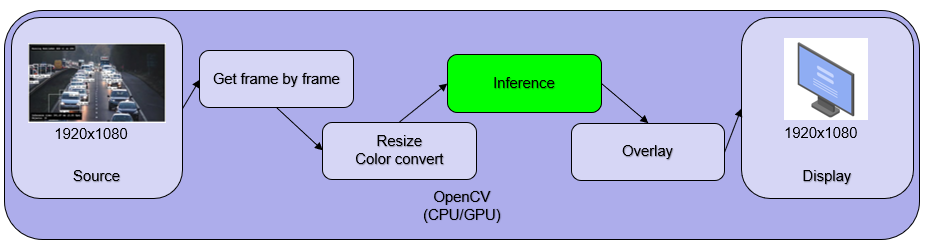
\includegraphics{../data/images/opencv_v4l2.png} For this approach, the
OpenCV needs to handle the entire process: open the video, get the
frame, resize and do a color convert on it, draw the informations at the
frame, and display the results. This is easely to test, but not fast for
ML purpose, once the entire process will be depent from OpenCV.

    The following code demonstrate the OpenCV V4L2 use case:

    \begin{tcolorbox}[breakable, size=fbox, boxrule=1pt, pad at break*=1mm,colback=cellbackground, colframe=cellborder]
\prompt{In}{incolor}{ }{\boxspacing}
\begin{Verbatim}[commandchars=\\\{\}]
\PY{k+kn}{from} \PY{n+nn}{ObjectDetection} \PY{k+kn}{import} \PY{n}{ObjectsDetectionOpenCV}


\PY{k}{def} \PY{n+nf}{main}\PY{p}{(}\PY{p}{)}\PY{p}{:}
    \PY{n}{app} \PY{o}{=} \PY{n}{ObjectsDetectionOpenCV}\PY{p}{(}\PY{p}{)}
    \PY{n}{app}\PY{o}{.}\PY{n}{run}\PY{p}{(}\PY{p}{)}


\PY{k}{if} \PY{n+nv+vm}{\PYZus{}\PYZus{}name\PYZus{}\PYZus{}} \PY{o}{==} \PY{l+s+s1}{\PYZsq{}}\PY{l+s+s1}{\PYZus{}\PYZus{}main\PYZus{}\PYZus{}}\PY{l+s+s1}{\PYZsq{}}\PY{p}{:}
    \PY{n}{main}\PY{p}{(}\PY{p}{)}
\end{Verbatim}
\end{tcolorbox}

    \textbf{GStreamer appsink pipeline + OpenCV V4L2 output}
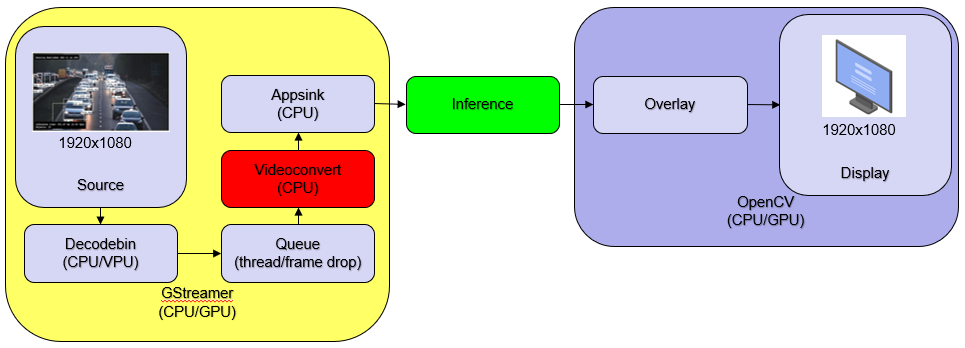
\includegraphics{../data/images/appsink_opencv_v4l2.png} This idea shows
a better perfomance than OpenCV V4L2 due the GStremaer usage at the
video openning process. It represents one less action to be processed by
the OpenCV, and the GStreamer pipelines enables a vast number of plugins
and its properties, which can guarantee some aditional chacateristics,
such as dropping frame property. It means that the displayed frame rate
will not be impacted for the inference process time. However, the
videoconvert usage, required for the appsink to be able to display the
results at screen, is a disavantage, once its only supported by CPU, and
resize/color convert by CPU has a high processing coast.

    The following code demonstrate this use case:

    \begin{tcolorbox}[breakable, size=fbox, boxrule=1pt, pad at break*=1mm,colback=cellbackground, colframe=cellborder]
\prompt{In}{incolor}{ }{\boxspacing}
\begin{Verbatim}[commandchars=\\\{\}]
\PY{k+kn}{from} \PY{n+nn}{ObjectDetection} \PY{k+kn}{import} \PY{n}{ObjectsDetectionV4L2}


\PY{k}{def} \PY{n+nf}{main}\PY{p}{(}\PY{p}{)}\PY{p}{:}
    \PY{n}{app} \PY{o}{=} \PY{n}{ObjectsDetectionV4L2}\PY{p}{(}\PY{p}{)}
    \PY{n}{app}\PY{o}{.}\PY{n}{run}\PY{p}{(}\PY{p}{)}


\PY{k}{if} \PY{n+nv+vm}{\PYZus{}\PYZus{}name\PYZus{}\PYZus{}} \PY{o}{==} \PY{l+s+s1}{\PYZsq{}}\PY{l+s+s1}{\PYZus{}\PYZus{}main\PYZus{}\PYZus{}}\PY{l+s+s1}{\PYZsq{}}\PY{p}{:}
    \PY{n}{main}\PY{p}{(}\PY{p}{)}
\end{Verbatim}
\end{tcolorbox}

    \textbf{GStreamer appsink + appsrc pipelines}
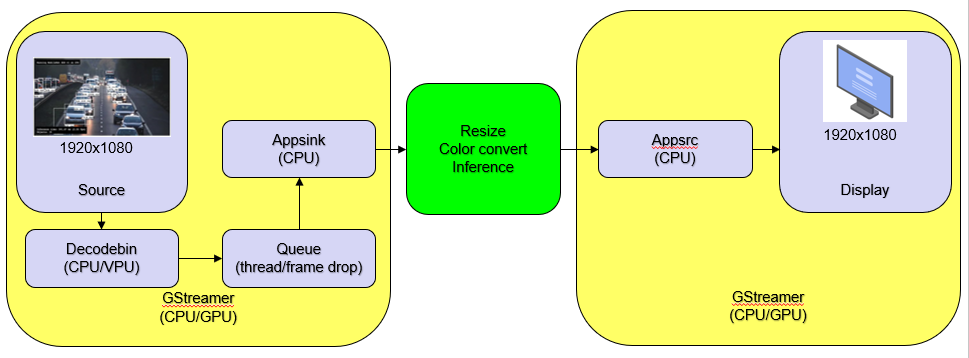
\includegraphics{../data/images/appsink_appsrc.png} This combination
shows very promissor, once we can use the appsink dropping frame
property, but do not requires videoconvert, once its results will not be
displayed yet. Actually, the resulted data will be processed by the
inference process, which can include resizing and color convert, and the
results will be send again to GStreamer, only to handle it and display
at the screen.

    The following code demonstrate this use case:

    \begin{tcolorbox}[breakable, size=fbox, boxrule=1pt, pad at break*=1mm,colback=cellbackground, colframe=cellborder]
\prompt{In}{incolor}{ }{\boxspacing}
\begin{Verbatim}[commandchars=\\\{\}]
\PY{k+kn}{from} \PY{n+nn}{ObjectDetection} \PY{k+kn}{import} \PY{n}{ObjectsDetectionAppsrc}


\PY{k}{def} \PY{n+nf}{main}\PY{p}{(}\PY{p}{)}\PY{p}{:}
    \PY{n}{app} \PY{o}{=} \PY{n}{ObjectsDetectionAppsrc}\PY{p}{(}\PY{p}{)}
    \PY{n}{app}\PY{o}{.}\PY{n}{run}\PY{p}{(}\PY{p}{)}


\PY{k}{if} \PY{n+nv+vm}{\PYZus{}\PYZus{}name\PYZus{}\PYZus{}} \PY{o}{==} \PY{l+s+s1}{\PYZsq{}}\PY{l+s+s1}{\PYZus{}\PYZus{}main\PYZus{}\PYZus{}}\PY{l+s+s1}{\PYZsq{}}\PY{p}{:}
    \PY{n}{main}\PY{p}{(}\PY{p}{)}
\end{Verbatim}
\end{tcolorbox}

    \textbf{GStreamer overlay plugins support:}
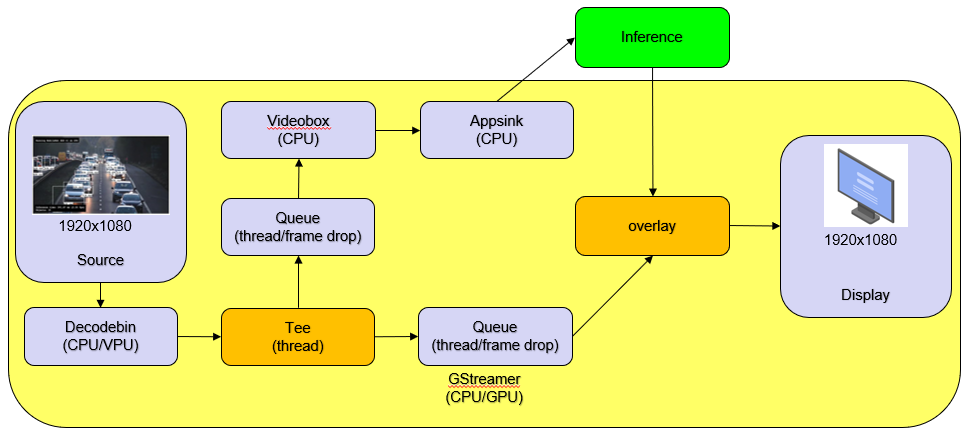
\includegraphics{../data/images/gstreamer_overlay.png}

This is the best approach, but the most dificult to use. Here, the tee
usage create two threads: one to be processed by the inference process;
other to be displayed. The videobox keeps the frame and is able to
return it ot the overlay plugin, so what we see is the combination of
two frames, one is the original video, without be touched, other is an
alpha image with all the required resizing process being displayed over
the original video.

    The following code demonstrate this use case:

    \begin{tcolorbox}[breakable, size=fbox, boxrule=1pt, pad at break*=1mm,colback=cellbackground, colframe=cellborder]
\prompt{In}{incolor}{ }{\boxspacing}
\begin{Verbatim}[commandchars=\\\{\}]
\PY{k+kn}{from} \PY{n+nn}{ObjectDetection} \PY{k+kn}{import} \PY{n}{ObjectsDetectionGStreamer}

\PY{k}{def} \PY{n+nf}{main}\PY{p}{(}\PY{p}{)}\PY{p}{:}
    \PY{n}{app} \PY{o}{=} \PY{n}{ObjectsDetectionGStreamer}\PY{p}{(}\PY{p}{)}
    \PY{n}{app}\PY{o}{.}\PY{n}{run}\PY{p}{(}\PY{p}{)}


\PY{k}{if} \PY{n+nv+vm}{\PYZus{}\PYZus{}name\PYZus{}\PYZus{}} \PY{o}{==} \PY{l+s+s1}{\PYZsq{}}\PY{l+s+s1}{\PYZus{}\PYZus{}main\PYZus{}\PYZus{}}\PY{l+s+s1}{\PYZsq{}}\PY{p}{:}
    \PY{n}{main}\PY{p}{(}\PY{p}{)}
\end{Verbatim}
\end{tcolorbox}

    \subsection{Results}\label{results}

The examples were made to return the FPS and inference time average
collected during the video playback process. With this values, two
graphs were generated: one showing the FPS per each example, other
showing the Inference time per each example.

    The code below generates de values to compose the graphs:

    \begin{tcolorbox}[breakable, size=fbox, boxrule=1pt, pad at break*=1mm,colback=cellbackground, colframe=cellborder]
\prompt{In}{incolor}{1}{\boxspacing}
\begin{Verbatim}[commandchars=\\\{\}]
\PY{k+kn}{from} \PY{n+nn}{ObjectDetection} \PY{k+kn}{import} \PY{n}{ObjectsDetectionOpenCV}
\PY{k+kn}{from} \PY{n+nn}{ObjectDetection} \PY{k+kn}{import} \PY{n}{ObjectsDetectionGStreamer}

\PY{n}{fps} \PY{o}{=} \PY{p}{[}\PY{p}{]}
\PY{n}{inf} \PY{o}{=} \PY{p}{[}\PY{p}{]}

\PY{n}{opencv} \PY{o}{=} \PY{n}{ObjectsDetectionOpenCV}\PY{p}{(}\PY{p}{)}
\PY{n}{inf\PYZus{}opencv}\PY{p}{,} \PY{n}{fps\PYZus{}opencv} \PY{o}{=} \PY{n}{opencv}\PY{o}{.}\PY{n}{run}\PY{p}{(}\PY{p}{)}

\PY{n}{fps}\PY{o}{.}\PY{n}{append}\PY{p}{(}\PY{n}{fps\PYZus{}opencv}\PY{p}{)}
\PY{n}{inf}\PY{o}{.}\PY{n}{append}\PY{p}{(}\PY{n}{inf\PYZus{}opencv}\PY{p}{)}

\PY{c+c1}{\PYZsh{}V4L2 is still not working, so I am simulating a value}
\PY{n}{fps}\PY{o}{.}\PY{n}{append}\PY{p}{(}\PY{l+m+mf}{1.5}\PY{p}{)}
\PY{n}{inf}\PY{o}{.}\PY{n}{append}\PY{p}{(}\PY{l+m+mi}{490}\PY{p}{)}

\PY{c+c1}{\PYZsh{}APPSRC is still not working, so I am simulating a value}
\PY{n}{fps}\PY{o}{.}\PY{n}{append}\PY{p}{(}\PY{l+m+mf}{2.25}\PY{p}{)}
\PY{n}{inf}\PY{o}{.}\PY{n}{append}\PY{p}{(}\PY{l+m+mi}{467}\PY{p}{)}

\PY{n}{gstreamer} \PY{o}{=} \PY{n}{ObjectsDetectionGStreamer}\PY{p}{(}\PY{p}{)}
\PY{n}{inf\PYZus{}gstreamer}\PY{p}{,} \PY{n}{fps\PYZus{}gstreamer} \PY{o}{=} \PY{n}{gstreamer}\PY{o}{.}\PY{n}{run}\PY{p}{(}\PY{p}{)}

\PY{n}{fps}\PY{o}{.}\PY{n}{append}\PY{p}{(}\PY{n}{fps\PYZus{}gstreamer}\PY{p}{)}
\PY{n}{inf}\PY{o}{.}\PY{n}{append}\PY{p}{(}\PY{n}{inf\PYZus{}gstreamer}\PY{p}{)}
\end{Verbatim}
\end{tcolorbox}

    \begin{Verbatim}[commandchars=\\\{\}]
Inference time: 0:00:00.471017
1.823114396716533
Inference time: 0:00:00.586821
1.624990069685684
Inference time: 0:00:00.470839
2.030042151247117
Inference time: 0:00:00.465317
2.090743149195542
Inference time: 0:00:00.466108
2.1007041831412727
Inference time: 0:00:00.471448
2.0683463114135714
Inference time: 0:00:00.478862
2.04182322873744
Inference time: 0:00:00.470132
2.074800134243718
Inference time: 0:00:00.470339
2.079438402244539
Inference time: 0:00:00.478474
2.0403286130412486
Inference time: 0:00:00.469643
2.080817711420963
Inference time: 0:00:00.471707
2.069075369447063
Inference time: 0:00:00.476293
2.050363892022392
Inference time: 0:00:00.471184
2.0747048089250812
Inference time: 0:00:00.472861
2.06630704507325
Inference time: 0:00:00.473493
2.0660335776446273
Inference time: 0:00:00.469347
2.079033121862539
Inference time: 0:00:00.471450
2.0738097766958132
Inference time: 0:00:00.472920
2.068800419834082
Inference time: 0:00:00.473172
2.066048005257613
Inference time: 0:00:00.474306
2.057072878109578
Inference time: 0:00:00.466973
2.092836813742929
Inference time: 0:00:00.469136
2.079698081744305
Inference time: 0:00:00.465397
2.099778298268023
Inference time: 0:00:00.472623
2.0697570422940053
Inference time: 0:00:00.467348
2.0915993251513343
Inference time: 0:00:00.481625
2.026425221181729
Inference time: 0:00:00.473435
2.065442918588161
Inference time: 0:00:00.466604
2.0924497489142952
Inference time: 0:00:00.473398
2.060624139148508
Inference time: 0:00:00.471572
2.0727938373733257
Inference time: 0:00:00.471134
2.076312891208623
Inference time: 0:00:00.481180
2.028254650081066
Inference time: 0:00:00.474473
2.0620897534298246
Inference time: 0:00:00.470228
2.077162839835135
Inference time: 0:00:00.470876
2.0752728998909085
Inference time: 0:00:00.470428
2.0740723582785114
Inference time: 0:00:00.467249
2.090165714921901
Inference time: 0:00:00.467497
2.085866870690033
Inference time: 0:00:00.473320
2.0604491353014076
Inference time: 0:00:00.471012
2.0750778651699355
Inference time: 0:00:00.472264
2.060615319887336
Inference time: 0:00:00.470608
2.071270075179357
Inference time: 0:00:00.476621
2.0550285770424397
Inference time: 0:00:00.471151
2.0732676061475646
Inference time: 0:00:00.470327
2.07783021300064
Inference time: 0:00:00.483831
2.0134643948047213
Inference time: 0:00:00.472028
2.070275990521167
Inference time: 0:00:00.471807
2.0675299356728996
Inference time: 0:00:00.473709
2.0619952523012954
Inference time: 0:00:00.474948
2.056208947248613
Inference time: 0:00:00.473496
2.0611914182320037
Inference time: 0:00:00.476927
2.0459961624886778
Inference time: 0:00:00.487019
2.002838707419251
Inference time: 0:00:00.467420
2.0910530962230514
Inference time: 0:00:00.464953
2.1029223485429216
Inference time: 0:00:00.468942
2.080081156779226
Inference time: 0:00:00.470416
2.0698880520710974
Inference time: 0:00:00.472206
2.0713025007141646
Inference time: 0:00:00.467141
2.0869327706294767
Inference time: 0:00:00.466024
2.0940749211801193
Inference time: 0:00:00.468406
2.0879957887797573
Inference time: 0:00:00.465525
2.0997077290829425
Inference time: 0:00:00.468244
2.0844011894326897
Inference time: 0:00:00.465749
2.1002381590263286
Inference time: 0:00:00.468781
2.084064349296454
Inference time: 0:00:00.466303
2.083833509812846
Inference time: 0:00:00.475887
2.0536497261675777
Inference time: 0:00:00.469499
2.0858277878212124
Inference time: 0:00:00.469025
2.079043910575814
Inference time: 0:00:00.467277
2.0869217692290003
Inference time: 0:00:00.464039
2.101944404512172
Inference time: 0:00:00.468105
2.089548294237787
Inference time: 0:00:00.474184
2.0591455119391564
Inference time: 0:00:00.473401
2.0565840472963655
Inference time: 0:00:00.476704
2.0542286874769977
Inference time: 0:00:00.488617
2.0043396599365977
Inference time: 0:00:00.562513
1.741814753071675
Inference time: 0:00:00.532090
1.8429854604038831
Inference time: 0:00:00.764878
1.2855791353509445
Inference time: 0:00:00.518767
1.883606148223827
Inference time: 0:00:00.609488
1.6044035744025913
Inference time: 0:00:00.601982
1.6259337499733286
Inference time: 0:00:00.467206
2.0854418758226014
Inference time: 0:00:00.535882
1.8169839500393081
Inference time: 0:00:00.615715
1.5849671646394168
Inference time: 0:00:00.620547
1.5802555413853163
Inference time: 0:00:00.663500
1.4739361360009835
Inference time: 0:00:00.578943
1.6938366735908281
Inference time: 0:00:00.610352
1.6088251110429996
Inference time: 0:00:00.542662
1.8001373591211602
Inference time: 0:00:00.504695
1.9312679205730068
Inference time: 0:00:00.503324
1.950238913042923
Inference time: 0:00:00.487535
2.0080741488769185
Inference time: 0:00:00.554387
1.7724861299371049
Inference time: 0:00:00.527378
1.8612238792537112
Inference time: 0:00:00.471896
2.0766494337920833
Inference time: 0:00:00.504275
1.9122041706132888
Inference time: 0:00:00.567001
1.731070543238274
Inference time: 0:00:00.549034
1.783099227412526
Inference time: 0:00:00.665034
1.4755565426700925
Inference time: 0:00:00.488863
2.002988811833286
Inference time: 0:00:00.477669
2.0536145656621727
Inference time: 0:00:00.469403
2.085651434965833
Inference time: 0:00:00.511931
1.9155335739649595
Inference time: 0:00:00.473390
2.0691883959451256
Inference time: 0:00:00.569518
1.7240075811992097
Inference time: 0:00:00.634755
1.528134160949401
Inference time: 0:00:00.482387
2.0268653749268513
Inference time: 0:00:00.475588
2.0484608563650424
Inference time: 0:00:00.465617
2.1036677672614656
Inference time: 0:00:00.467323
2.0978497147414235
Inference time: 0:00:00.472480
2.074560810912296
Inference time: 0:00:00.475793
2.0606294766003397
Inference time: 0:00:00.472337
2.0674007415423272
Inference time: 0:00:00.465517
2.1058480383455893
Inference time: 0:00:00.590202
1.66760800915306
Inference time: 0:00:00.463501
2.1126644262691405
Inference time: 0:00:00.568532
1.721197523245646
Inference time: 0:00:00.458199
2.1382056048561147
Inference time: 0:00:00.462043
2.1141776525045772
Inference time: 0:00:00.467192
2.097041822422788
Inference time: 0:00:00.463766
2.1076386530163145
Inference time: 0:00:00.474842
2.0648325583607217
Inference time: 0:00:00.465280
2.1069791349311715
Inference time: 0:00:00.468553
2.094626490236417
Inference time: 0:00:00.465564
2.098630539900366
Inference time: 0:00:00.486998
2.014760948643665
Inference time: 0:00:00.463634
2.1145086756927105
Inference time: 0:00:00.462572
2.1194499976389327
Inference time: 0:00:00.465284
2.0997230629058428
Inference time: 0:00:00.467876
2.0956499483327984
Inference time: 0:00:00.462823
2.115504685734988
Inference time: 0:00:00.463697
2.111859517753289
Inference time: 0:00:00.474978
2.0552634570599673
Inference time: 0:00:00.464199
2.108918246202497
Inference time: 0:00:00.472253
2.06692511718804
Inference time: 0:00:00.463344
2.1138868594694253
Inference time: 0:00:00.464779
2.096984378351309
Inference time: 0:00:00.464835
2.0989674618630785
Inference time: 0:00:00.473841
2.0613365405586115
Inference time: 0:00:00.465969
2.0948222682296866
Inference time: 0:00:00.482671
2.032455204016593
Inference time: 0:00:00.468108
2.085821562020206
Inference time: 0:00:00.468038
2.0925962148378887
Inference time: 0:00:00.464487
2.1111811185807303
Inference time: 0:00:00.461979
2.1228422852538156
Inference time: 0:00:00.465869
2.0966008858138743
Inference time: 0:00:00.466384
2.097589218267241
Inference time: 0:00:00.463458
2.1139699995101933
Inference time: 0:00:00.464284
2.112658257936099
Inference time: 0:00:00.461585
2.119792204740588
Inference time: 0:00:00.462773
2.1175963062682928
Inference time: 0:00:00.466874
2.1014302287905684
Inference time: 0:00:00.468934
2.0877168820246492
Inference time: 0:00:00.466044
2.104743640698624
Inference time: 0:00:00.465036
2.1042945134743882
Inference time: 0:00:00.467610
2.0956361144156963
Inference time: 0:00:00.462861
2.1188244461946972
Inference time: 0:00:00.462354
2.119929598494789
Inference time: 0:00:00.466011
2.1022839162010794
Inference time: 0:00:00.463874
2.1038462816467236
Inference time: 0:00:00.465885
2.0960877653746675
Inference time: 0:00:00.462469
2.12009276491334
Inference time: 0:00:00.463676
2.112817485662299
Inference time: 0:00:00.465549
2.104572751695873
Inference time: 0:00:00.467909
2.087890650552193
Inference time: 0:00:00.474647
2.0648950679175995
Inference time: 0:00:00.462886
2.115876863964532
Inference time: 0:00:00.471290
2.0740103328231787
Inference time: 0:00:00.469333
2.080500398294117
Inference time: 0:00:00.467140
2.089008385739242
Inference time: 0:00:00.465900
2.095353854558472
Inference time: 0:00:00.471976
2.076522965290161
Inference time: 0:00:00.472810
2.0755575983931416
Inference time: 0:00:00.462772
2.1135641253770467
Inference time: 0:00:00.463542
2.1064200436938503
Inference time: 0:00:00.465659
2.1036153671913005
Inference time: 0:00:00.463191
2.110899040577177
Inference time: 0:00:00.462038
2.1216832306865463
Inference time: 0:00:00.462748
2.111213232371795
Inference time: 0:00:00.469147
2.08357905675676
Inference time: 0:00:00.463334
2.1142807030779998
Inference time: 0:00:00.471819
2.079208158357051
Inference time: 0:00:00.465279
2.100460527861148
Inference time: 0:00:00.463753
2.1147106566916527
Inference time: 0:00:00.460679
2.1285914718144454
Inference time: 0:00:00.462302
2.118753650453633
Inference time: 0:00:00.477009
2.0554114973589925
Inference time: 0:00:00.499076
1.9676201308482735
Inference time: 0:00:00.469955
2.085850685688579
Inference time: 0:00:00.467992
2.0872560702102847
Inference time: 0:00:00.462443
2.1174203827438496
Inference time: 0:00:00.464225
2.103513946551991
Inference time: 0:00:00.478640
2.0412235756285244
Inference time: 0:00:00.462733
2.110809204650448
Inference time: 0:00:00.460802
2.116832987116478
Inference time: 0:00:00.466058
2.094382957479766
Inference time: 0:00:00.466200
2.102707283990405
Inference time: 0:00:00.463581
2.1048395046617205
Inference time: 0:00:00.465923
2.1025027134742333
Inference time: 0:00:00.483219
2.0304043178838116
Inference time: 0:00:00.594967
1.6476078014090998
Inference time: 0:00:00.585403
1.6795603322206616
Inference time: 0:00:00.472863
2.0690074224896438
Inference time: 0:00:00.468655
2.0831026253777756
Inference time: 0:00:00.467447
2.0957552941125974
Inference time: 0:00:00.471706
2.0769679889593364
Inference time: 0:00:00.468715
2.0838994550104872
Inference time: 0:00:00.466232
2.095975488958384
Inference time: 0:00:00.464018
2.106958230187281
Inference time: 0:00:00.465002
2.1073414268829453
Inference time: 0:00:00.525265
1.8695379124649558
Inference time: 0:00:00.486975
2.000343867112132
Inference time: 0:00:00.502517
1.9414917294442355
Inference time: 0:00:00.512423
1.9083879472774472
Inference time: 0:00:00.510092
1.915378442502971
Inference time: 0:00:00.484457
2.0240940340814078
Inference time: 0:00:00.509020
1.9197562947709845
Inference time: 0:00:00.501215
1.955602591882927
Inference time: 0:00:00.502601
1.9516600999386977
Inference time: 0:00:00.841902
1.1704136028306003
Inference time: 0:00:00.520857
1.885205003507518
Inference time: 0:00:00.526717
1.8644261807534521
Inference time: 0:00:00.493128
1.9816047158641201
Inference time: 0:00:00.557408
1.7503198276280834
Inference time: 0:00:00.535766
1.821430103641595
Inference time: 0:00:00.698736
1.4070041295908884
Inference time: 0:00:00.690488
1.423880460496667
Inference time: 0:00:00.618025
1.5851950216373334
Inference time: 0:00:00.561492
1.7271727343344456
Inference time: 0:00:00.508867
1.9272978239142382
Inference time: 0:00:00.509995
1.9191764368660476
Inference time: 0:00:00.474589
2.0623449773949463
Inference time: 0:00:00.491958
1.981110868614336
Inference time: 0:00:00.554980
1.7704685972533751
Inference time: 0:00:00.491126
1.9959189485178035
Inference time: 0:00:00.586566
1.6759963292864715
Inference time: 0:00:00.629707
1.5440041809162812
Inference time: 0:00:00.629461
1.5646590265399076
Inference time: 0:00:00.546397
1.7962652333485594
Inference time: 0:00:00.595784
1.6494721456558328
Inference time: 0:00:00.479665
2.033238971864818
Inference time: 0:00:00.476007
2.0586502116504457
Inference time: 0:00:00.472258
2.066821598920636
Inference time: 0:00:00.490376
1.9965486701344695
Inference time: 0:00:00.480171
2.0340150203140945
Inference time: 0:00:00.476606
2.0479175768551006
Inference time: 0:00:00.470095
2.0821109953716506
Inference time: 0:00:00.604311
1.6241773955656695
Inference time: 0:00:00.545512
1.7869739012801242
Inference time: 0:00:00.496132
1.9716490082659708
Inference time: 0:00:00.469278
2.080571967875894
Inference time: 0:00:00.474364
2.059460161245557
Inference time: 0:00:00.471957
2.069747493537855
Inference time: 0:00:00.503292
1.9492612710102368
Inference time: 0:00:00.500592
1.9573236695305216
Inference time: 0:00:00.572777
1.7144260062556422
Inference time: 0:00:00.503836
1.9485072357465467
Inference time: 0:00:00.529410
1.8536603137482832
Inference time: 0:00:00.527406
1.8228927995882072
Inference time: 0:00:00.469047
2.0883581143893815
Inference time: 0:00:00.570412
1.7179896666288812
Inference time: 0:00:00.484093
2.0174566733123167
Inference time: 0:00:00.473889
2.0611039153851216
Inference time: 0:00:00.473400
2.062753367609377
Inference time: 0:00:00.559085
1.7555821261739963
Inference time: 0:00:00.489001
1.9995216624307834
Inference time: 0:00:00.491114
1.9910056875546311
Inference time: 0:00:00.533617
1.8286371140525137
Inference time: 0:00:00.470146
2.086391492089406
Inference time: 0:00:00.467614
2.0951752112479265
Inference time: 0:00:00.474223
2.0550248184525315
Inference time: 0:00:00.465397
2.1058188768463824
Inference time: 0:00:00.463970
2.1138061789940927
Inference time: 0:00:00.465524
2.097261667519665
Inference time: 0:00:00.489263
1.9946891123128196
Inference time: 0:00:00.525189
1.825088623839704
Inference time: 0:00:00.469792
2.0741505804241798
Inference time: 0:00:00.509972
1.9221903127951463
Inference time: 0:00:00.545709
1.7928187044015276
Inference time: 0:00:00.589536
1.661886143153287
Inference time: 0:00:00.565183
1.7382289922502348
Inference time: 0:00:00.570922
1.7159069355154914
Inference time: 0:00:00.596764
1.6439343831153077
Inference time: 0:00:00.490028
1.9950837823763168
Inference time: 0:00:00.520332
1.8785196119560823
Inference time: 0:00:00.546600
1.7685938894561153
Inference time: 0:00:00.489696
1.9967034545767146
Inference time: 0:00:00.490597
1.9942665037443998
Inference time: 0:00:00.534834
1.8257397267035962
Inference time: 0:00:00.624856
1.5724760287115378
Inference time: 0:00:00.487707
2.010197353255965
Inference time: 0:00:00.465515
2.1047869664603143
Inference time: 0:00:00.464398
2.111900554556364
Inference time: 0:00:00.473556
2.061070754864814
Inference time: 0:00:00.479285
2.045118437676108
Inference time: 0:00:00.467401
2.0971345144062172
Inference time: 0:00:00.486850
2.0163989288808235
Inference time: 0:00:00.465528
2.1037921952498904
Inference time: 0:00:00.478151
2.050677036355313
Inference time: 0:00:00.466990
2.090264323225348
Inference time: 0:00:00.495816
1.9781534982745546
Inference time: 0:00:00.466707
2.091545188554336
Inference time: 0:00:00.470340
2.076976970321503
Inference time: 0:00:00.462852
2.1093002920442268
Inference time: 0:00:00.467161
2.097165749276889
Inference time: 0:00:00.459198
2.1273828834291892
Inference time: 0:00:00.464870
2.100382333646385
Inference time: 0:00:00.461448
2.122709064649945
Inference time: 0:00:00.460806
2.123855437579327
Inference time: 0:00:00.475801
2.055349729636419
Inference time: 0:00:00.463328
2.117177518665831
Inference time: 0:00:00.462709
2.1119561113217813
Inference time: 0:00:00.462658
2.120282650978882
Inference time: 0:00:00.465381
2.103222151268621
Inference time: 0:00:00.478221
2.041845862717886
Inference time: 0:00:00.508269
1.9050173004527144
Inference time: 0:00:00.642824
1.5293041616056449
Inference time: 0:00:00.582887
1.6809727929409686
Inference time: 0:00:00.474605
2.0664426615269003
Inference time: 0:00:00.473571
2.069061841345199
Inference time: 0:00:00.540559
1.8111858821972644
Inference time: 0:00:00.487002
1.9943383963755101
Inference time: 0:00:00.488648
2.0047334804668715
Inference time: 0:00:00.479874
2.043205333942808
Inference time: 0:00:00.487070
2.0108182059697537
Inference time: 0:00:00.522036
1.8728331460962153
Inference time: 0:00:00.478036
2.0477484900916267
Inference time: 0:00:00.468553
2.0867190959291184
Inference time: 0:00:00.475035
2.0647214737084965
Inference time: 0:00:00.471895
2.0418599753358015
Inference time: 0:00:00.470373
2.0735956718982167
Inference time: 0:00:00.475547
2.055101817389012
Inference time: 0:00:00.495549
1.9735880591338533
Inference time: 0:00:00.612460
1.5724326862834155
Inference time: 0:00:00.610880
1.6090416918406603
Inference time: 0:00:00.476902
2.0490762616678913
Inference time: 0:00:00.495724
1.9711856497180078
Inference time: 0:00:00.518587
1.890102485893031
Inference time: 0:00:00.515412
1.8897360554628462
Inference time: 0:00:00.534694
1.835009569923559
Inference time: 0:00:00.521131
1.8775799650276324
Inference time: 0:00:00.494431
1.9726473429578508
Inference time: 0:00:00.526748
1.8647620936427693
Inference time: 0:00:00.472379
2.0708346340159385
Inference time: 0:00:00.513388
1.9060117292950323
Inference time: 0:00:00.466954
2.0985659623677133
Inference time: 0:00:00.506532
1.9311578754894998
Inference time: 0:00:00.477862
2.0511346052079897
Inference time: 0:00:00.469859
2.0773197738916362
Inference time: 0:00:00.467513
2.094740425610784
Inference time: 0:00:00.506123
1.9400574813810987
Inference time: 0:00:00.472881
2.055409385002952
Inference time: 0:00:00.497364
1.9717742488057703
Inference time: 0:00:00.505350
1.9415448679913356
Inference time: 0:00:00.489639
2.0020769185579272
Inference time: 0:00:00.558549
1.7526004678261997
Inference time: 0:00:00.581890
1.6872420320821784
Inference time: 0:00:00.728272
1.350945894150863
Inference time: 0:00:00.657060
1.486355317638293
Inference time: 0:00:00.627449
1.5361139640246348
Inference time: 0:00:00.548197
1.7801878831654148
Inference time: 0:00:00.657098
1.4955998868046252
Inference time: 0:00:00.498497
1.961038606600334
Inference time: 0:00:00.468869
2.09231204148407
Gstreamer pipeline:
 filesrc location=../data/video/Home-And-Away.mp4 ! qtdemux name=demux
demux.video\_0
                    ! queue ! decodebin  ! videorate
                    ! videoconvert n-threads=4 ! videoscale n-threads=4
                    ! video/x-raw,width=640,height=480,framerate=30/1 ! queue
max-size-buffers=1 leaky=downstream  ! tee name=t
            t. ! queue max-size-buffers=1 leaky=downstream ! videoconvert !
videoscale ! video/x-raw,width=300,height=225 ! videobox name=box autocrop=true
               ! video/x-raw,format=RGB,width=300,height=300 ! appsink
name=appsink emit-signals=true max-buffers=1 drop=true sync=false
            t. ! queue ! videoconvert
               ! rsvgoverlay name=overlay ! videoconvert ! ximagesink

Inference time: 0:00:00.758688
Inference time: 0:00:00.496941
Inference time: 0:00:00.470070
    \end{Verbatim}

    The code below generates de FPS graph:

    \begin{tcolorbox}[breakable, size=fbox, boxrule=1pt, pad at break*=1mm,colback=cellbackground, colframe=cellborder]
\prompt{In}{incolor}{3}{\boxspacing}
\begin{Verbatim}[commandchars=\\\{\}]
\PY{k+kn}{from} \PY{n+nn}{ObjectDetection} \PY{k+kn}{import} \PY{n}{graphs}

\PY{n}{fps\PYZus{}g} \PY{o}{=} \PY{n}{graphs}\PY{p}{(}\PY{p}{)}
\PY{n}{fps\PYZus{}g}\PY{o}{.}\PY{n}{start}\PY{p}{(}\PY{n}{fps}\PY{p}{,} \PY{l+s+s1}{\PYZsq{}}\PY{l+s+s1}{FPS}\PY{l+s+s1}{\PYZsq{}}\PY{p}{)}
\end{Verbatim}
\end{tcolorbox}

    \begin{center}
    \adjustimage{max size={0.9\linewidth}{0.9\paperheight}}{output_20_0.png}
    \end{center}
    { \hspace*{\fill} \\}
    
    The code below generates de Inference graph:

    \begin{tcolorbox}[breakable, size=fbox, boxrule=1pt, pad at break*=1mm,colback=cellbackground, colframe=cellborder]
\prompt{In}{incolor}{6}{\boxspacing}
\begin{Verbatim}[commandchars=\\\{\}]
\PY{k+kn}{from} \PY{n+nn}{ObjectDetection} \PY{k+kn}{import} \PY{n}{graphs}

\PY{n}{inf\PYZus{}g} \PY{o}{=} \PY{n}{graphs}\PY{p}{(}\PY{p}{)}
\PY{n}{inf\PYZus{}g}\PY{o}{.}\PY{n}{start}\PY{p}{(}\PY{n}{inf}\PY{p}{,} \PY{l+s+s1}{\PYZsq{}}\PY{l+s+s1}{Inference*1000 (ms)}\PY{l+s+s1}{\PYZsq{}}\PY{p}{)}
\end{Verbatim}
\end{tcolorbox}

    \begin{center}
    \adjustimage{max size={0.9\linewidth}{0.9\paperheight}}{output_22_0.png}
    \end{center}
    { \hspace*{\fill} \\}
    
    \subsection{Conclusion}\label{conclusion}

Unfortunately, the object detection algorithms consume a lot of process
resources, and the notebooks have no performance enough to handle it.
However, it was still able to show the difference at the inference time
and the framerate, both running together and consuming the same CPU
process. According to the values obtained, noticed that the number of
about 0.5 milliseconds is far from the expected for a video object
detection solution. With some simples calculations, it is easy to note
that 0.5 ms of inference time represents 2 frames being calculated per
second. It is very slow and it is far from the multimedia capabilities,
which can achieve 60 frames per second.

    \subsection{Source}\label{source}

Martín Abadi, Paul Barham, Jianmin Chen, Zhifeng Chen, Andy Davis,
Jeffrey Dean, Matthieu Devin, Sanjay Ghemawat, Geoffrey Irving, Michael
Isard, et al. 2016. TensorFlow: A System for Large-Scale Machine
Learning.

Ganesh Ananthanarayanan, Paramvir Bahl, Peter Bodík, Krishna
Chintalapudi, Matthai Philipose, Lenin Ravindranath, and Sudipta Sinha.
2017. Real-Time Video Analytics: The Killer App for Edge Computing.

Google. 2019. Coral Edge TPU. Retrieved June 16, 2020, from
https://coral.ai/

Nvidia. 2020. NVIDIA DeepStream SDK. Retrieved June 16, 2020 from
https://developer.nvidia.com/deepstream-sdk

GStreamer. 2019. GStreamer: open source multimedia framework. Retrieved
June 16, 2020 from https://gstreamer.freedesktop.org

Intel. 2020.03. Intel's Deep Learning Inference Engine Developer Guide.
Retrieved June 16, 2020 from
https://docs.openvinotoolkit.org/latest/\_docs\_IE\_DG\_Deep\_Learning\_Inference\_Engine\_DevGuide.html


    % Add a bibliography block to the postdoc
    
    
    
\end{document}
